Text-attributed graphs (TAGs) associate graph relations with text
at each node and arise naturally in Web content networks. Examples
include academic citation networks, product and purchase networks,
online knowledge communities, and linked document collections. In these
networks, graph structure supplies relational context, while node text such
as titles, descriptions, or posts supplies semantics that topology alone
cannot express. The networks are continuously updated as new content,
relations, and sometimes new classes arrive. Retraining on the accumulated
graph can preserve historical information, but its storage and training cost
grow with the entire history.

Graph condensation replaces a large training graph with a much smaller set of
training items. In the continual setting, each arriving increment must be
converted into useful memory before its raw data leaves the access
window. A later stage may receive only the current increment and the memory
written by earlier stages. For TAGs, every retained item must also carry a
readable text. The memory is therefore not merely a smaller training
set. It is the interface through which released graph and text information is
carried to future stages.

\noindent\textbf{Research gap.}
Existing studies provide complementary pieces of this problem. Static TAG
condensation uses a fully available source graph to construct compact data
that combines graph and text information~\cite{tagsam,stad}, while continual graph condensation
studies how to preserve graph training utility under a limited replay
budget~\cite{cat,puma,gecc}. Federated and multimodal condensation methods
consider related settings with different access boundaries~\cite{dance,srgm},
and graph and language alignment methods target transferable TAG prediction
rather than continual memory construction~\cite{graphclip}. These lines of
work do not explicitly define an interface in which the current graph is
converted into a compact memory before release and new memory rows are added
over time. Each retained row must preserve graph information and readable
text. This paper studies continual TAG condensation with limited access to
historical raw data.

\noindent\textbf{Two challenges.}
The access boundary and the requirement to retain text create two coupled challenges,
visualized in~\autoref{fig:challenge_overview}.

\emph{(i) Preserving graph information after source data become unavailable.}
Neighborhood information is produced from the current graph and cannot be
recovered from an isolated node feature or text string after the raw
increment is released. Later stages cannot recompute the released
neighborhoods or jointly recondense those nodes with future data. The
constructor must therefore decide what relational evidence to commit to a
small memory while classes and graph patterns continue to change. The
memory must carry this information into later stages. This makes the
balance between preserving earlier knowledge and learning new information
central to continual condensation.

\emph{(ii) Coordinating continuous feature construction with discrete text selection.}
Condensation combines information from multiple nodes, but the stored text
must be a real and readable source string. A continuous pooled representation
need not correspond to an actual string. Selecting text only after feature optimization can
break the correspondence between a synthetic feature and its text, whereas
storing an optimized text vector loses provenance and auditability. A
continual TAG condenser must coordinate feature construction and text
selection so that the retained features and readable texts describe
compatible source information.

\begin{figure}[t]
\centering
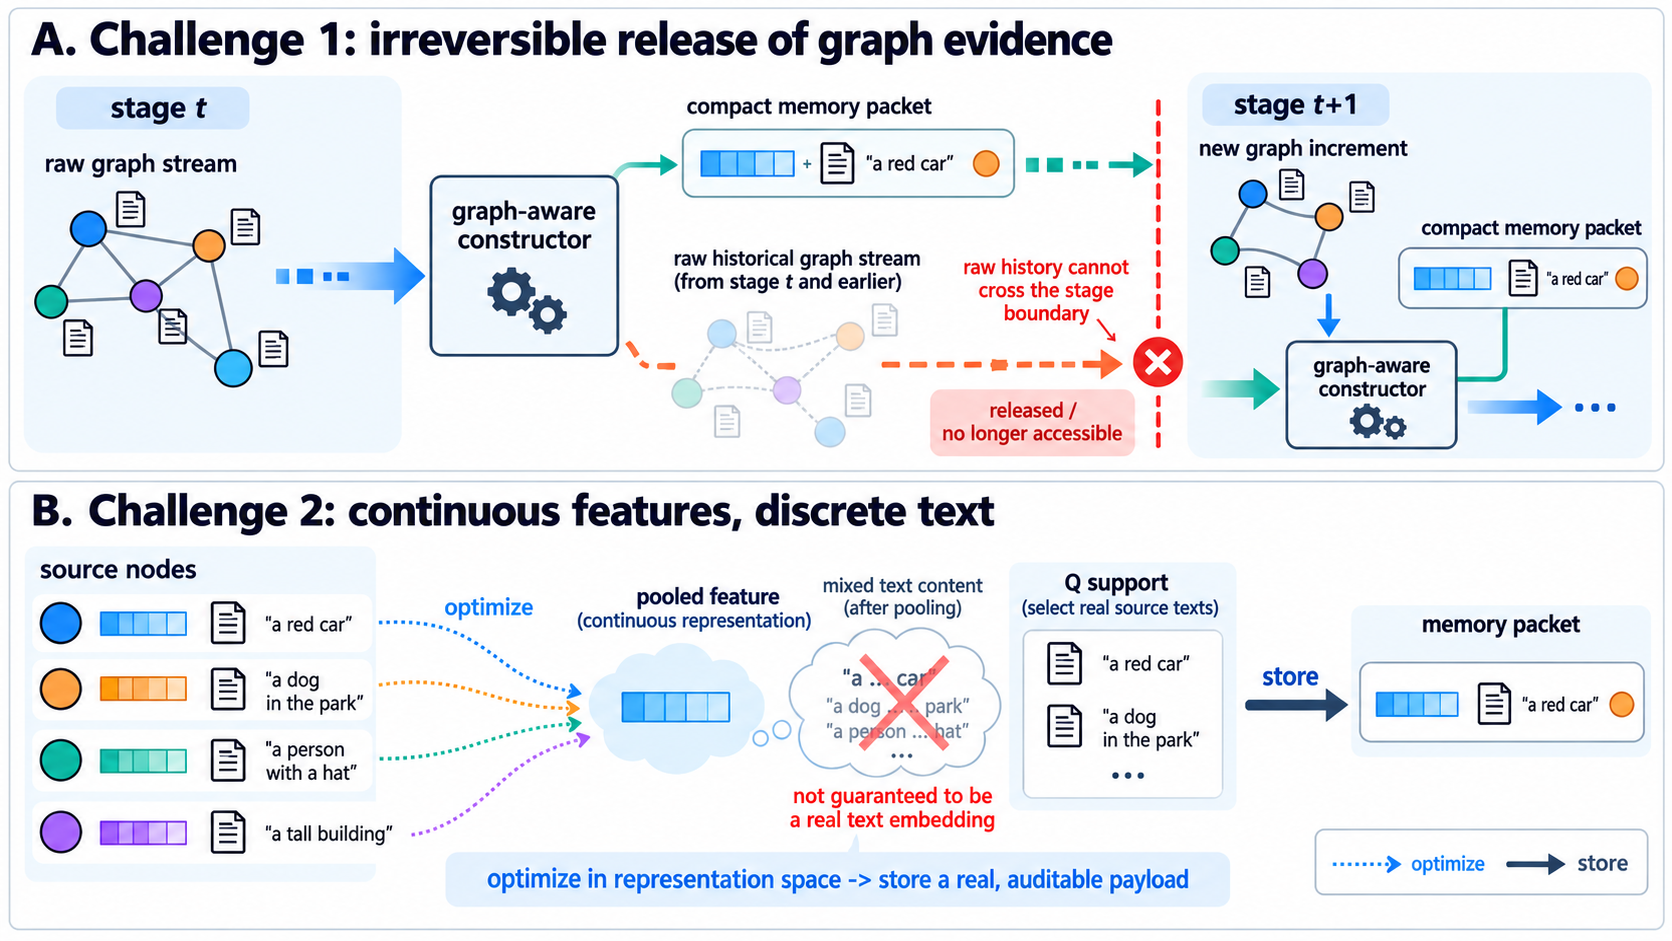
\includegraphics[width=\columnwidth]{challenge_overview_v2.png}
\caption{Information flow in the two challenges. Only the compact memory
crosses the stage boundary after the raw increment is released. The
lower panel shows the conversion from continuous feature construction to a
real, auditable text.}
\Description{Two compact panels visualize irreversible release of a raw graph
increment and the mismatch between continuous feature construction and
discrete text selection.}
\label{fig:challenge_overview}
\end{figure}

\noindent\textbf{Design principles and CoTAG-Q.}
The two challenges motivate three design principles. Graph information
should be extracted before release. Feature construction and text selection
should use one auditable support matrix. The text rule used during
construction should also agree with the text that is ultimately stored.

We propose \method{} around these principles. At each stage, the current
graph is used to construct new memory items, historical memory
is kept fixed, and only new items are appended. A support matrix constrained
by class labels coordinates feature aggregation with text selection.
Neighborhood summaries guide numerical features, and training feedback
refines the source contributions used by both features and text.
Algorithmic details are given in~\autoref{sec:method_interface}.

Under a fixed condensation rate, \method{} improves recognition of
historical classes on BookHis and retains high training utility relative
to all observed raw data on the two product graphs. The same memories
also train a GraphSAGE student without further construction. Chronological
streams extend the evaluation to document arrivals with recurring classes.
Training on the condensed memory also reduces the cost of subsequent student
updates, while construction remains a separate upfront cost.
The experiments report the detailed comparisons, robustness checks, and
limitations of these results.

\noindent\textbf{Contributions.}
\begin{itemize}[leftmargin=*,nosep]
\item We formulate continual TAG condensation with an explicit historical
access boundary. Each stage receives the current increment and a stored
condensed memory. Each retained item contains numerical features that
preserve graph information together with readable text.
\item We propose \method{}, which learns a support matrix constrained by
class labels for feature aggregation and text selection
before the current source is released.
\item We establish a consistent construction and storage interface for readable
text and evaluate memory retention, architecture transfer, construction cost,
and a separate topology extension under the same continual protocol. We also
measure downstream reuse: under a common student budget, condensed memories
reduce peak GPU allocation by 89.5--93.8\% and training time by 50.9--88.4\%
relative to the full observed training pool.
\end{itemize}
